%!TEX root=main.tex
\section{实现}
\label{clicknp:sec:impl}

\subsection{\name 工具链和硬件实现}

\textbf{图:编译生成的 OpenCL 代码示例,(1)只包含顺序和选择结构,不包含分支结构,(2)非阻塞(每个流水级有最坏时钟周期数的保证)。可以避免 handler 阻塞 signal。}

我们构建了一个\name 编译器,它作为\name 工具链的前端(\S \ref {clicknp:subsec:toolchain})。
对于宿主程序,我们使用Visual C++作为后端。我们进一步集成了Altera OpenCL SDK(v15.1)\cite {aoc}和Xilinx Vivado HLS(v2015.4)\cite {vivado}作为FPGA程序的后端。
\name 编译器包含4,925行C ++代码,它们解析配置文件和元素声明,在\S \ref {clicknp:sec:optimization}中执行优化,并生成特定于每个商业HLS工具的代码。
使用Altera OpenCL时,每个\name 元素都被编译成\textit {kernel},元素之间的连接被转换为Altera扩展通道。
使用Xilinx Vivado HLS时,我们将每个元素编译成IP内核,并使用AXI流来实现元素之间的连接。
元素也可以编译为CPU二进制文件,管理器线程将为每个主机元素创建一个工作线程。
主机和FPGA元素之间的每个连接都映射到PCIe I / O通道的\textit {插槽}(\S \ref {clicknp:subsec:pcie})。

\textbf{图:ClickNP element,channel,signal 菊花链,command hub 的示例}

我们的硬件平台基于Altera Stratix V FPGA和Catapult shell \cite {putnam2014reconfigurable}。
Catapult shell还包含一个OpenCL特定的运行时,因此\name role可以通过此运行时层与shell通信。
FPGA板具有PCIe Gen2 x8接口,4GB板载DDR内存和两个40G以太网端口。
到撰写本文时,我们还没有获得Xilinx硬件平台。
因此,主系统评估基于使用\name + OpenCL的Altera平台,我们使用Vivado HLS生成的报告(例如频率和面积成本)来了解\name + Vivado的性能。

\subsection{\name 元件库}
\label{clicknp:subsec:lib}

我们已经实现了一个包含近100个元素的\name 元件库。
其中一部分(20%)直接来自Click Modular Router,但使用\name 编程框架重新编写。
这些元素涵盖了网络功能的大量基本操作,包括数据包解析,校验和计算,封装/解封,哈希表,最长前缀匹配(LPM),速率限制,加密和数据包调度。
由于\name 的模块化体系结构,每个元素的代码大小都是适中的。
元素的平均代码行数(Line of Code,LoC)是80,最复杂的元素\textit {PacketBuffer}有196行C代码。
表 \ref {clicknp:tab:elements}显示了我们在\name 中实现的一组选定的关键元素。
除了元素名称,我们还标记了使用该元素的演示网络功能(A1 至 A5,在\S \ref {clicknp:sec:application}中讨论)。
我们已经大量应用了之前在\S \ref {clicknp:subsec:paral_in_elem}中讨论的优化技术,以最小化内存依赖性和平衡管道阶段。
我们总结了第3列中每个元素使用的优化技术。
对于表 \ref {clicknp:tab:elements}顶部的元件,元件中的处理逻辑需要访问数据包的每个字节。我们以Gbps显示吞吐量。
但是,表格底部的元素只处理数据包头(元数据)。因此,使用每秒数据包来测量吞吐量更有意义。
我们注意到表 \ref {clicknp:tab:elements}中测量的吞吐量是相应元素可以实现的最大吞吐量。
当它们在真正的网络功能中工作时,其他组件,例如以太网端口,可能是瓶颈。
作为参考,我们将优化版本与我们之前在FPGA上的实现进行比较,而不应用\S \ref {clicknp:sec:optimization} 中讨论的技术以及CPU实现。
很明显,经过优化后,所有这些元素都可以非常有效地处理数据包,与我们的初始FPGA实现相比,速度提高了7倍~117倍,与一个CPU内核上的软件实现相比,速度提高了21%。
这种性能提升来自于利用FPGA中的巨大并行性的能力。
考虑到FPGA的功耗(大约30W)和CPU(每个核心大约5W),\name 元件的能耗效率比CPU高4到120倍。

我们还显示了表 \ref {clicknp:tab:elements} 中每个元素的处理延迟。
我们看到,这个延迟很低:平均值是 $0.19 \mu s$,最大值仅为$0.8 \mu s$(LPM \_Tree)。
最后两列总结了每个元素的资源利用率。 利用率归一化为FPGA芯片的容量。
我们可以看到大多数元素只使用少量的逻辑元素。
这是合理的,因为大多数数据包操作都很简单。
HashTCAM和RateLimiter具有适度的逻辑资源使用,因为这些元素具有更大的仲裁逻辑。
但是,BRAM的使用很大程度上依赖于元素的配置。 例如,BRAM使用率随流表中支持的条目数呈线性增长。
总的来说,我们的FPGA芯片有足够的容量来支持包含少量元素的有意义的网络功能(\S \ref{clicknp:sec:application})。



\subsection{PCIE I/O 通道}
\label{clicknp:subsec:pcie}

如前所述,\name 的一个关键属性是支持联合CPU / FPGA处理。
我们通过设计高吞吐量,低延迟的PCIe I / O通道来实现这一目标。
我们扩展OpenCL运行时并添加一个新的I / O通道,它连接到shell中的PCIe开关。
PCIe交换机将仲裁新添加的I / O通道与shell中的其他组件(例如DDR内存控制器)之间的访问。

我们利用Catapult shell \cite {putnam2014reconfigurable}中的PCIe插槽DMA引擎,它将PCIe Gen2 x8链路划分为64个逻辑子通道,即\textit {slots}。
每个插槽都有一对用于DMA操作的发送和接收缓冲区。
在64个插槽中,33个由Shell保留,运行时库用于控制内核和访问板载DDR,一个插槽用于将信号传递给\name 元件。
然而,剩余的30个插槽用于FPGA和CPU元件之间的数据通信。
为了分摊DMA开销,我们积极地使用\textit {batching}。最大邮件大小限制为64KB。
PCIe通道可以在中断或轮询模式下工作。


在FPGA中,一个名为\textit {CmdHub}的特殊元素由\name 编译器自动生成,使用FIFO缓冲区将数据从不同的插槽重定向到相应的FPGA元素。
\textit {CmdHub}还用于将控制信号从管理器线程分发到FPGA元素。
为了识别目标元素,在信号消息中嵌入元素ID,并且\textit {CmdHub}可以读取ID并再次通过FIFO缓冲器将信号消息转发到相应的元素。

图 \ref {clicknp:fig:pcie} 显示了具有不同插槽数和批量大小的PCIe I / O通道的基准。
作为基线,我们还测量OpenCL全局内存操作的性能 - 到目前为止,这是OpenCL \cite {opencl}中为CPU / FPGA通信提供的唯一方法。
我们可以看到单个插槽的最大吞吐量约为8.4~Gbps。
通过4个插槽,PCIe I / O通道的总吞吐量可达25.6~Gbps。
这是由于DMA引擎时钟频率的限制,我们可以从当前FPGA芯片中获得的最大吞吐量。
但是,OpenCL的吞吐量低得惊人,低于1~Gbps。这是因为全局内存API旨在传输 GB 级的大量数据。这可能适用于具有大数据集的应用程序,但不适用于需要强流处理功能的网络功能。
同样,图 \ref {clicknp:fig:pcie}(b)显示了通信延迟。由于OpenCL未针对流处理进行优化,因此OpenCL延迟高达1~ms,通常是网络功能无法接受的。
相比之下,PCIe I / O通道在轮询模式下具有非常低的1 $\mu$s的延迟(一个 CPU 核重复轮询状态寄存器),而在中断模式下的延迟为 9 $\mu$ s(几乎没有CPU开销) 。

\begin{figure}[htbp]
	\centering
	\subfloat[]{
		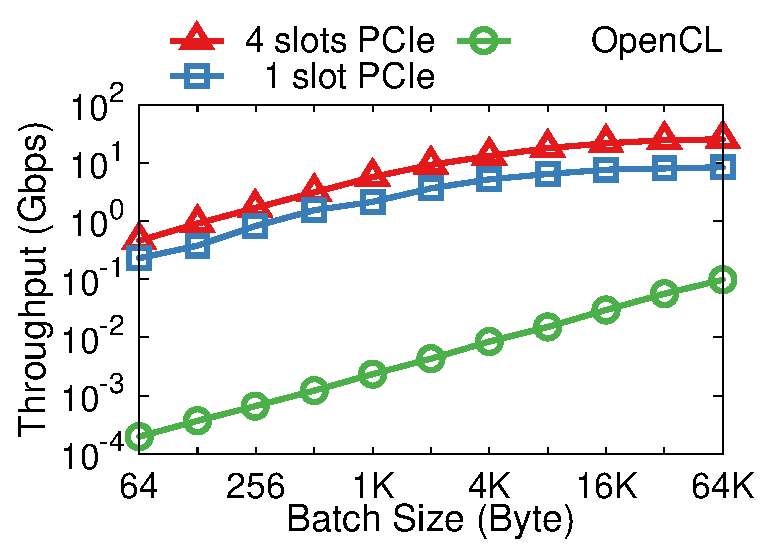
\includegraphics[width=0.5\textwidth]{eval/pcie_1}
	}
	\subfloat[]{
		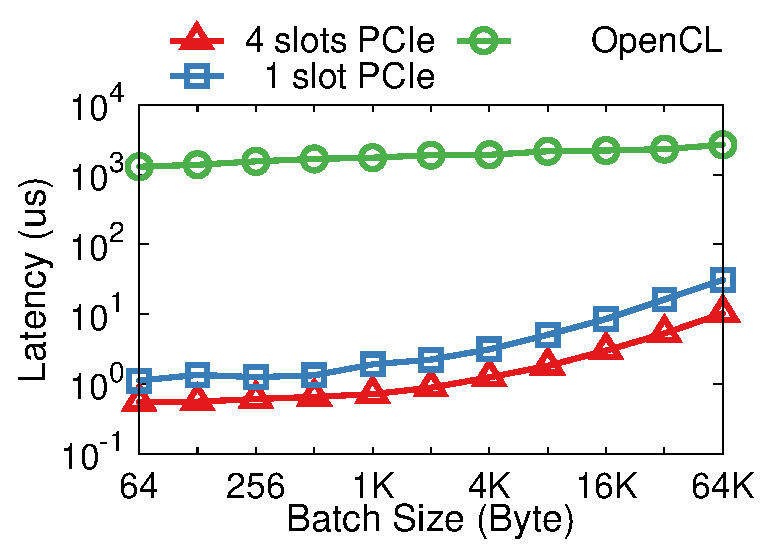
\includegraphics[width=0.5\textwidth]{eval/pcie_2}
	}

	\caption{PCIe I/O 通道的性能。Y 轴是对数坐标系。}

	\label{clicknp:fig:pcie}
\end{figure}

\iffalse
\subsection{Verilog 元件}

\textbf{把 Verilog 元件封装成一个 OpenCL kernel,使用 Avalon ST 或 AXI 接口与外部连接。}

\subsection{元件热迁移和高可用}

\textbf{虚拟机热迁移,计算节点对应的网卡状态;网络、存储节点热迁移(升级,扩容等),网卡状态;高可用性,故障恢复……}

\textbf{热升级:不丢包,的时候原来的 FPGA 不处理了,buffer 起来。把旧 FPGA 的状态迁移到新 FPGA,让交换机开始往新 FPGA 的 buffer 里灌,然后从旧 FPGA 的 buffer 里把数据倒出来在新的 FPGA 里处理,处理完后开始处理新 FPGA 自己的 buffer,迁移结束。}

\textbf{高可用:状态机复制的方法,两个 FPGA 收到相同的数据包序列,只要元件内部没有随机化或与时间相关的处理逻辑,就能保证两个 FPGA 收到的数据包序列相同。检测到备份节点故障,只需启动一个新的备份节点,然后执行热升级操作。检测到主节点故障,切换输出到备份节点(可能出现少量数据包丢失或重复,TCP 可以安全地处理这些情况)。}

\fi

\egg{

\egg{
Control signals can only be generated by the manager thread. 
When the manager thread sends a signal to a target element in FPGA, it will embed the ID of the element in the signal message, and 
passes the message to \textit{CmdHub} through slot 32.
\textit{CmdHub} will parse the message and forward the signal request to corresponding elements, again through FIFO buffers. 
}



\egg{
As aforementioned, OpenCL advocates batch processing model where communication between host program and a kernel in FPGA must go through shared DRAM, and the host program cannot control the kernel while it is running.
We could use a special kernel to proxy messages between host program and the kernel via DRAM, but it incurs \approx1ms latency.
DDR access is performed via PCIe link and raw PCIe latency is merely \approx1$\mu$s. As we improve kernel communication efficiency with channels in place of shared memory, we design a host-kernel communication mechanism with channel abstraction for low latency and high throughput.
We leverage I/O channel in Altera OpenCL and AXI stream in Vivado HLS to connect the Catapult shell to kernels and built a PCIe bypass switch to arbitrate accesses for on-board DRAM and kernel I/O channel.

A PCIe link is split into multiple logically independent \textit{slots} which can operate in parallel.
One slot is reserved for signals. Remaining slots are assigned to channels between host and FPGA elements, so each channel can transfer data in parallel without head-of-line blocking.
On CPU side, each host element is run on a separate core and receives input flits via PCIe by polling or interrupt.
On FPGA side, each element that communicates with host is connected to an inbound demultiplexer and an outbound multiplexer, where load-adaptive batching is performed to improve peak throughput while preserving low latency under light load.
}

\egg{
With polling model, the latency of the PCIe I/O channel  is $< 2 \mu s$ when message size is small, but the latency will reach to $32 \mu s$
for full batched messages.
The interrupt model, however, will increase the latency.
}

\egg{
, where each slot is assigned to one CPU core. Our PCIe channel has two bottlenecks: (1) PCIe Gen2 x8 interface has 32 Gbps bandwidth, (2) PCIe data width is 128b and the clock frequency of Catapult shell is 200 MHz, which limits PCIe throughput to 25.6 Gbps. PCIe I/O channel offers 1\approx2$\mu$s RTT which translates to 400\approx800K host-kernel transactions per second. Polling mode yields lower latency and higher throughput, while interrupt mode latency can be improved by utilizing more cores and PCIe slots. Four CPU cores are sufficient to saturate maximum throughput for both polling and interrupt mode under 64KB batch size. Effectiveness of batching will be further evaluated in traffic dumper application.
}

}
